
\chapter{背景分析}

排序算法是一种重要的算法,许多时候,我们希望一套数据能够以某种方式排序,而排序算法使这种%
需求得以实现。经过排序的数据能够以更快的方式查找、筛选和计算。排序算法在很多领域得到相当地重视,%
尤其是在大量数据的处理方面,一个优秀的算法可以节省大量的资源。%

排序算法要求一个序列经过排序之后能够按照既定模式排列,而且对于不同方式打乱的数据,相同模式的排序算法%
应该给出相同的排列。从头到尾逐个两两比较可以判定一个序列是否是良序的。此外,需要说明的是,这种排列模式中%
两个元素的关系需要满足偏序关系或是全序关系。

排序算法十分被重视,著名计算机领域图书%
\emph{《计算机程序设计艺术》(The Art Of Computer Programming, TAOCP) \footnote{作者 Donald E.Knuth 是 \LaTeX 之父}}就用了%
一卷的容量来讨论排序。


\chapter{功能设计}

\section{题意转化}
本题的指向明确,需要比较八种不同算法在排序过程中主键的交换、比较次数。并且给不同的样本容量以计时。

要实现排序算法,首先介绍这几种排序算法(下文中的 $n$ 指代数组大小):

\section{冒泡排序}
\subsubsection{描述}

最简单的排序,顺序遍历整个序列,发现两个元素逆序就交换这两个元素的位置,重复 $n$ 次。

\begin{figure}[H]
    \centering
    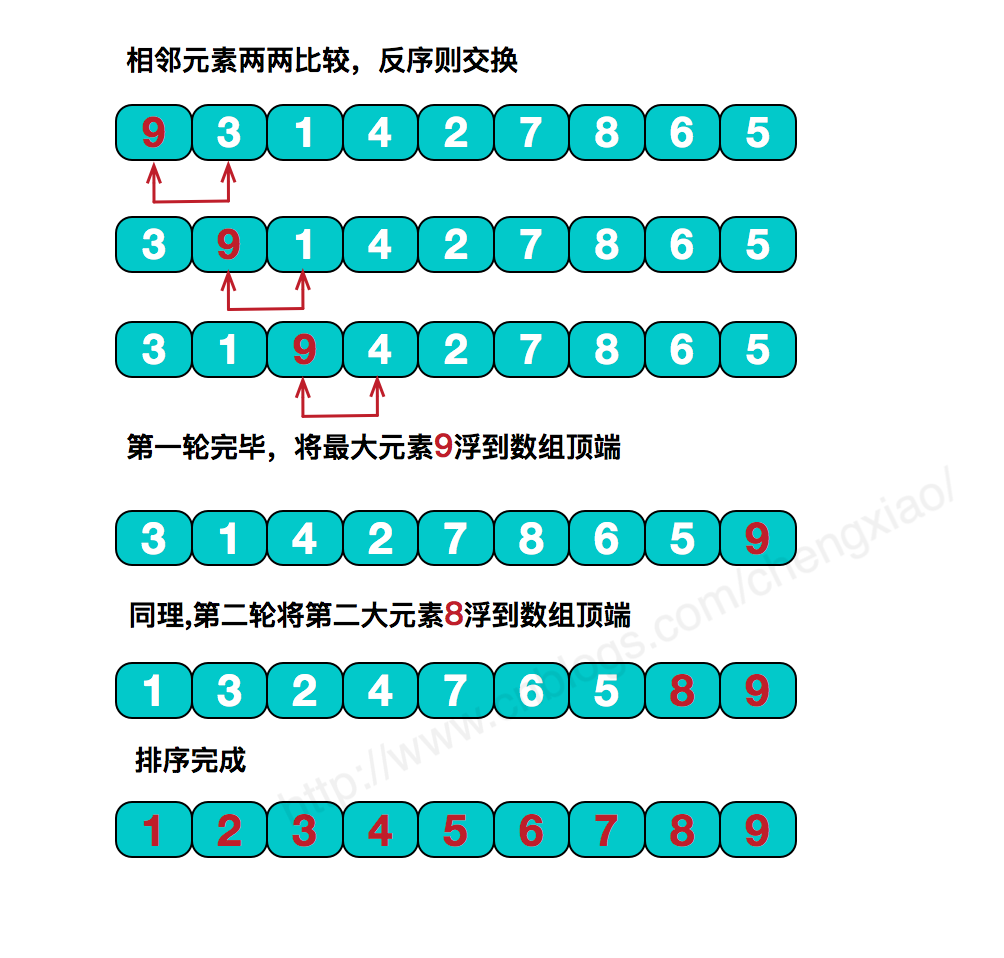
\includegraphics[width=10.5cm]{src/bubble.png}
    \caption{冒泡排序示意图}
\end{figure}


可以证明,在第 $i$ 次遍历之后,第 $i$ 小的元素会出现在 $i$ 位置上,$i$之前的元素都已排序,所以第$i$次遍历序列时只要从 $i$ 位置开始就行。%
当一次遍历没有出现元素交换,说明数组已经良序,可以退出返回,不用做接下来的排序。

\subsubsection{性能}
\begin{itemize}
    \item 冒泡排序的时间复杂度为 $O(n)$。
    \item 最好情况下冒泡排序只需要 $n$次比较,没有交换,此时数组有序。
    \item 数据比较次数和输入序列中个排序元素的初始排列无关,数据的移动次数和各排序元素的初始序列有关。 
    \item 冒泡排序是稳定的。
\end{itemize}


\section{选择排序}

\subsubsection{描述}
在 $i$ 从 $0$ 增加到 $n$ 的过程中,每次从 $i$ 位置开始向后遍历数组,找到遍历元素中最小的与 $i$ 位置元素交换。

\begin{figure}[H]
    \centering
    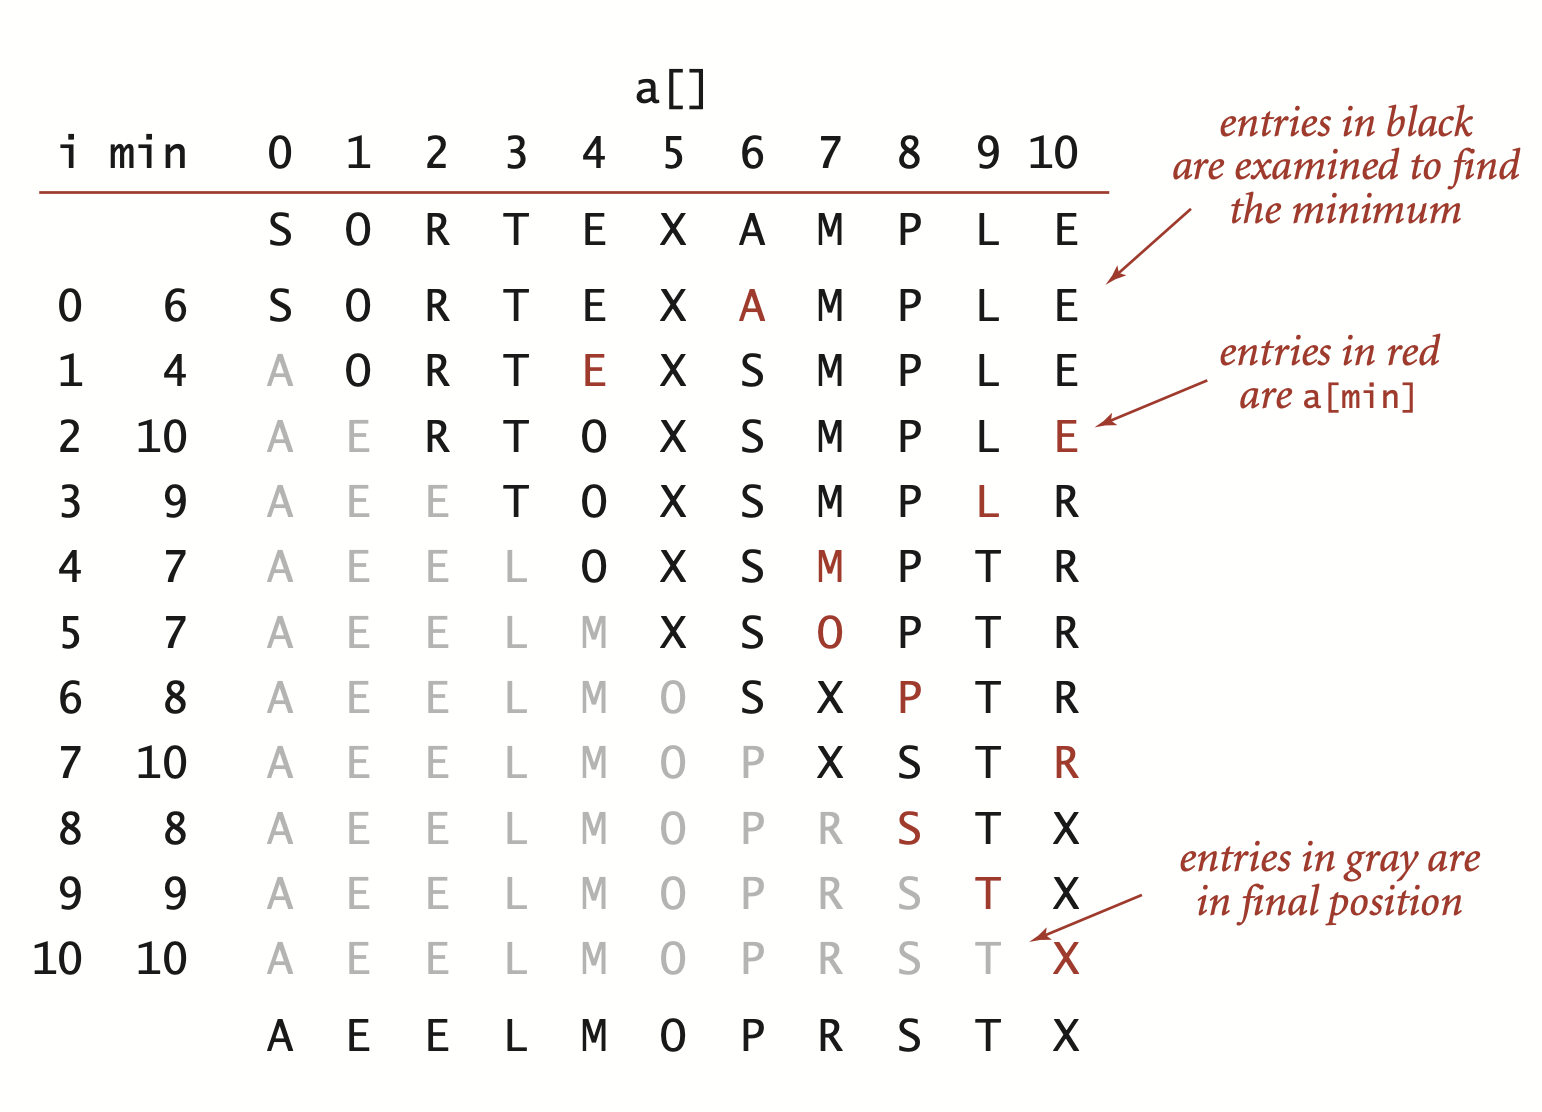
\includegraphics[width=14.5cm]{src/selection.png}
    \caption{选择排序示意图}
\end{figure}

\subsubsection{性能}
\begin{itemize}
    \item 选择排序的时间复杂度为 $O(n)$。
    \item 数据比较次数和输入序列中个排序元素的初始排列无关,数据的移动次数和各排序元素的初始序列有关。 
    \item 选择排序是稳定的。
\end{itemize}


\section{直接插入排序}

\subsubsection{描述}
在 $i$ 从 $0$ 增加到 $n$ 的过程中,每次取 $i$ 位置的元素,向前找到第一个比 $i$ 位置元素小的元素,将 $i$ 位置元素插入在这个元素之后。

\begin{figure}[H]
    \centering
    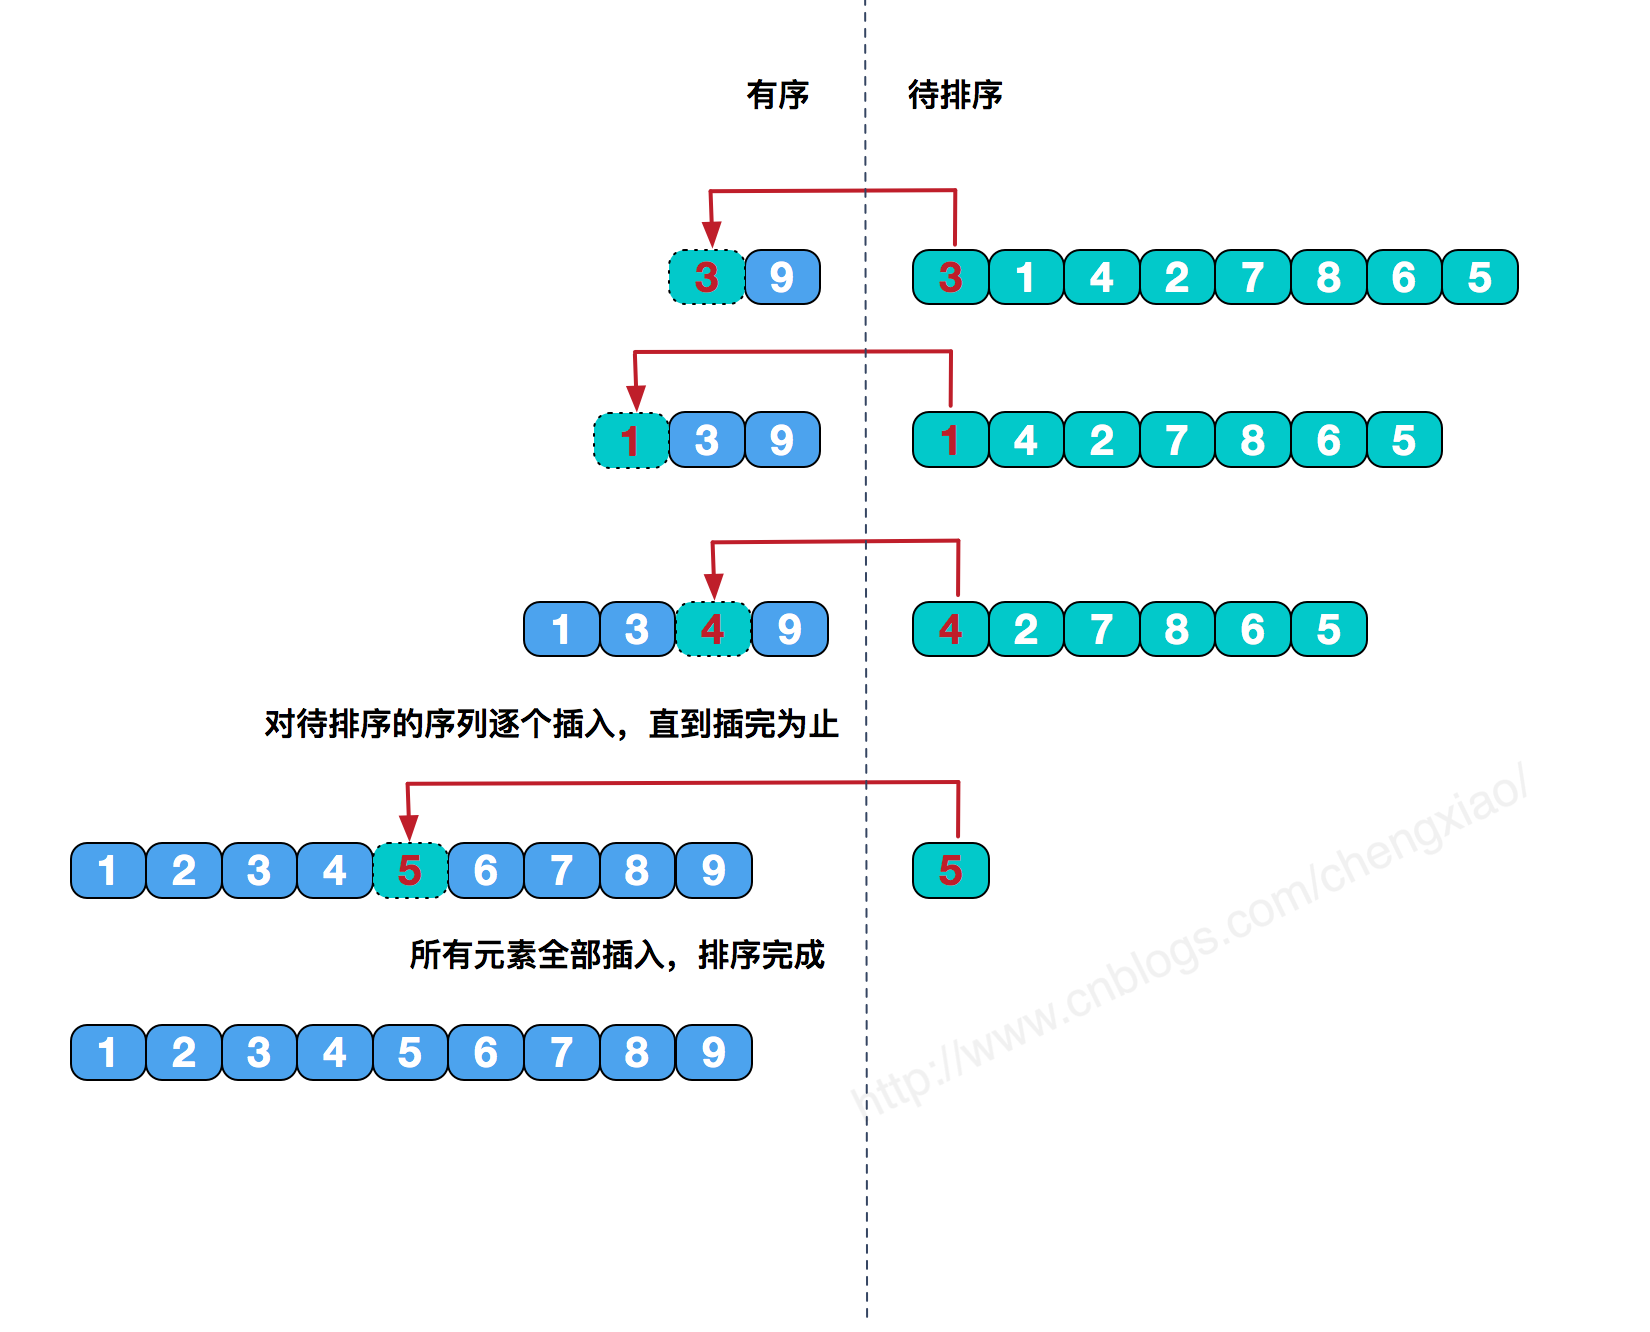
\includegraphics[width=13.5cm]{src/insertion.png}
    \caption{直接插入排序示意图}    
\end{figure}

因为是在数组中实现,插入这个动作需要以些调整:数组中插入某位置后原先在这个位置的元素和之后的元素都要向后移动,所以在插入时边让比 $i$ 位置%
元素大的元素向后移动,一边比较,找到  $i$ 元素应该放的位置就直接覆盖。这样的直接插入排序算法主键交换次数为 $0$ (项目会用{\kaishu 赋值次数}记录)

\subsubsection{性能}
\begin{itemize}
    \item 直接插入排序的时间复杂度为 $O(n)$。
    \item 数据比较次数和移动次数与输入序列中个排序元素的初始排列有关。
    \item 直接插入排序是稳定的。
\end{itemize}

\section{希尔排序}

\subsubsection{描述}
选定一个比 $\frac{n}{2}$ 小的值定为 $\text{gap}$,将元素划分为 $\text{gap}$ 个子序列,%
以$\text{gap}$为步长从 $0$ 到 $n - \text{gap}$ 用插入排序对间隔的字串排序。%
之后将 $\text{gap}$ 减小继续重复排序步骤,直到 $\text{gap}$ 减小为 $1$,完成后数组有序。


\begin{figure}[H]
    \centering
    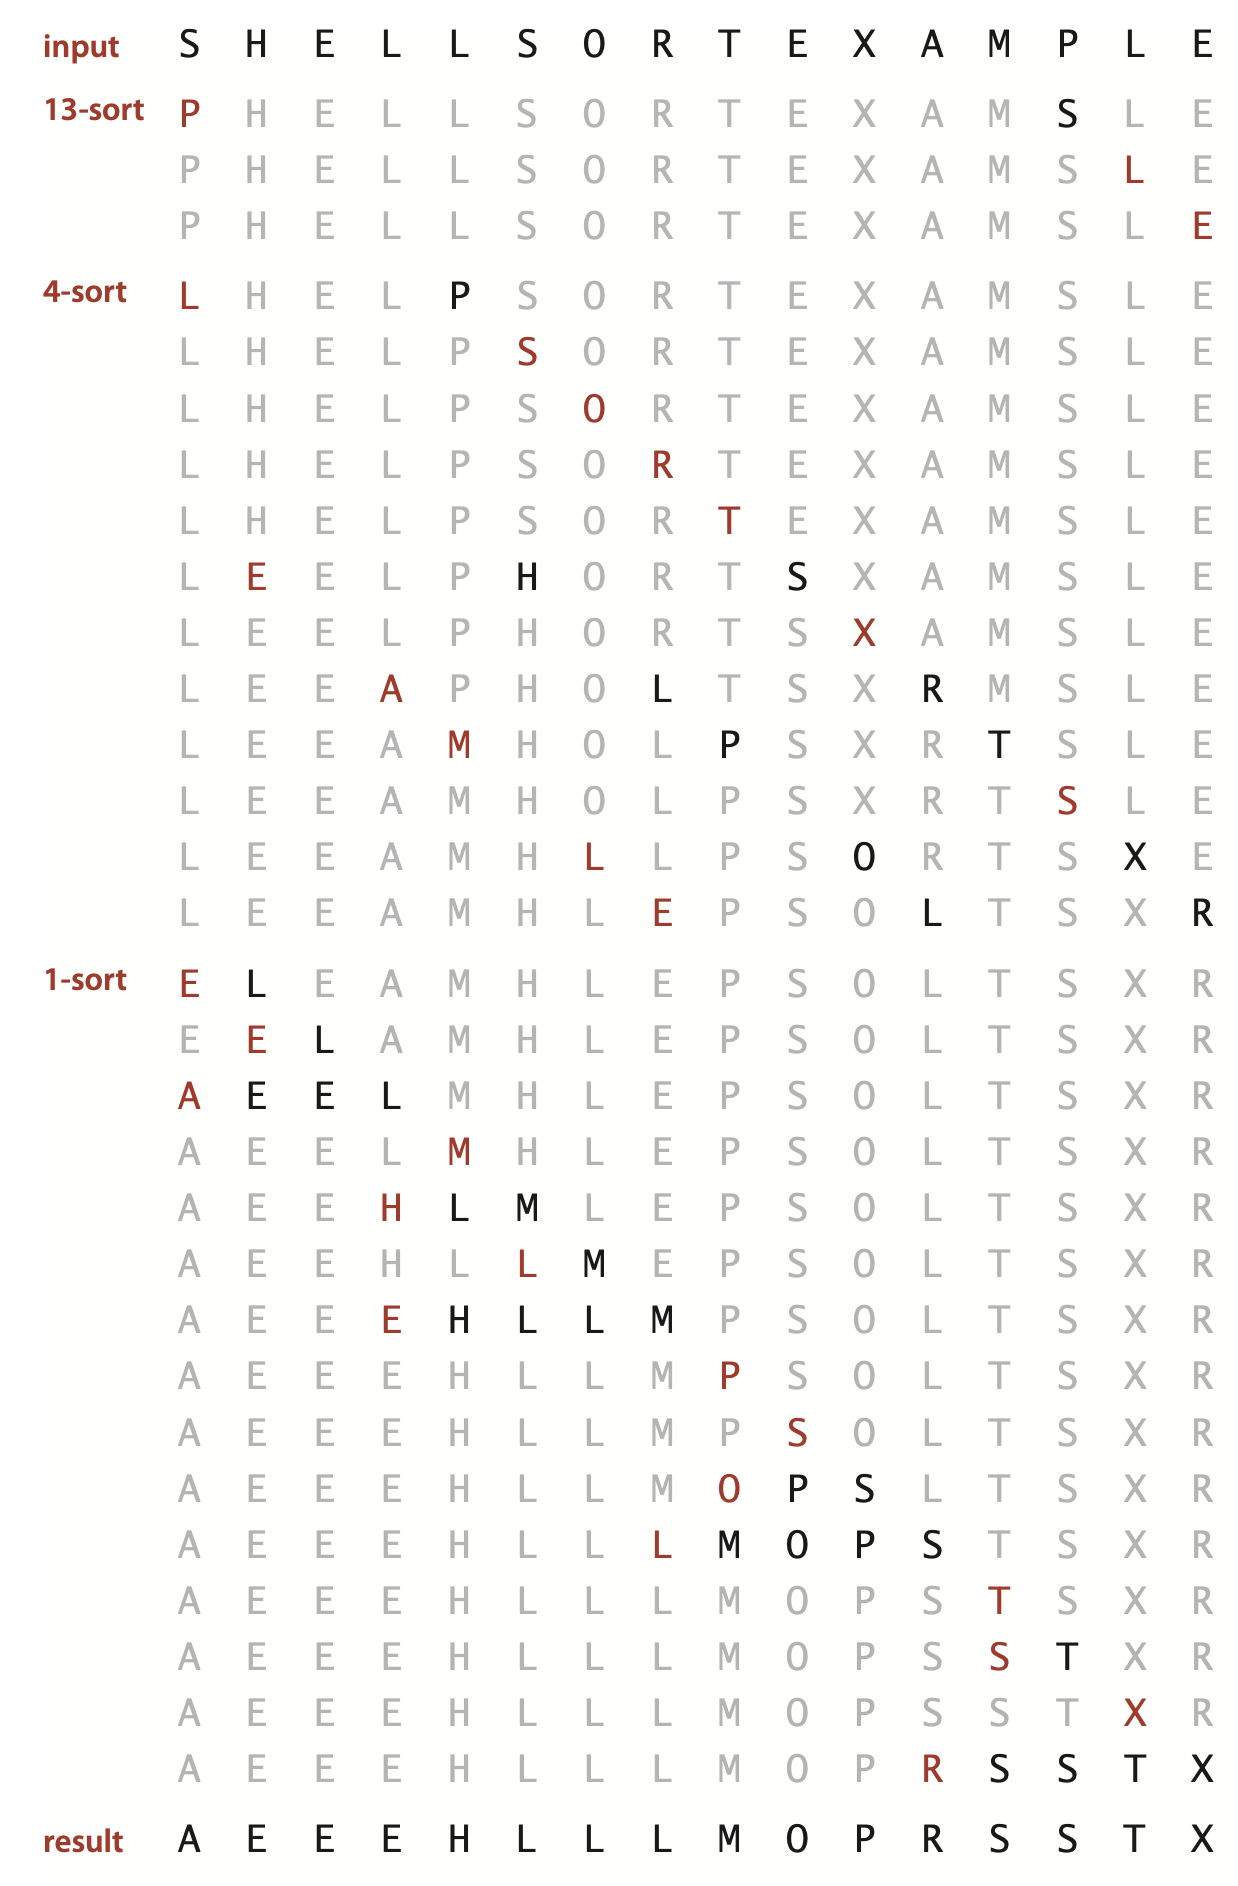
\includegraphics[width=12.5cm]{src/shellString.png}
    \caption{希尔排序示意图}
\end{figure}

\newpage

\begin{figure}[H]
    \centering
    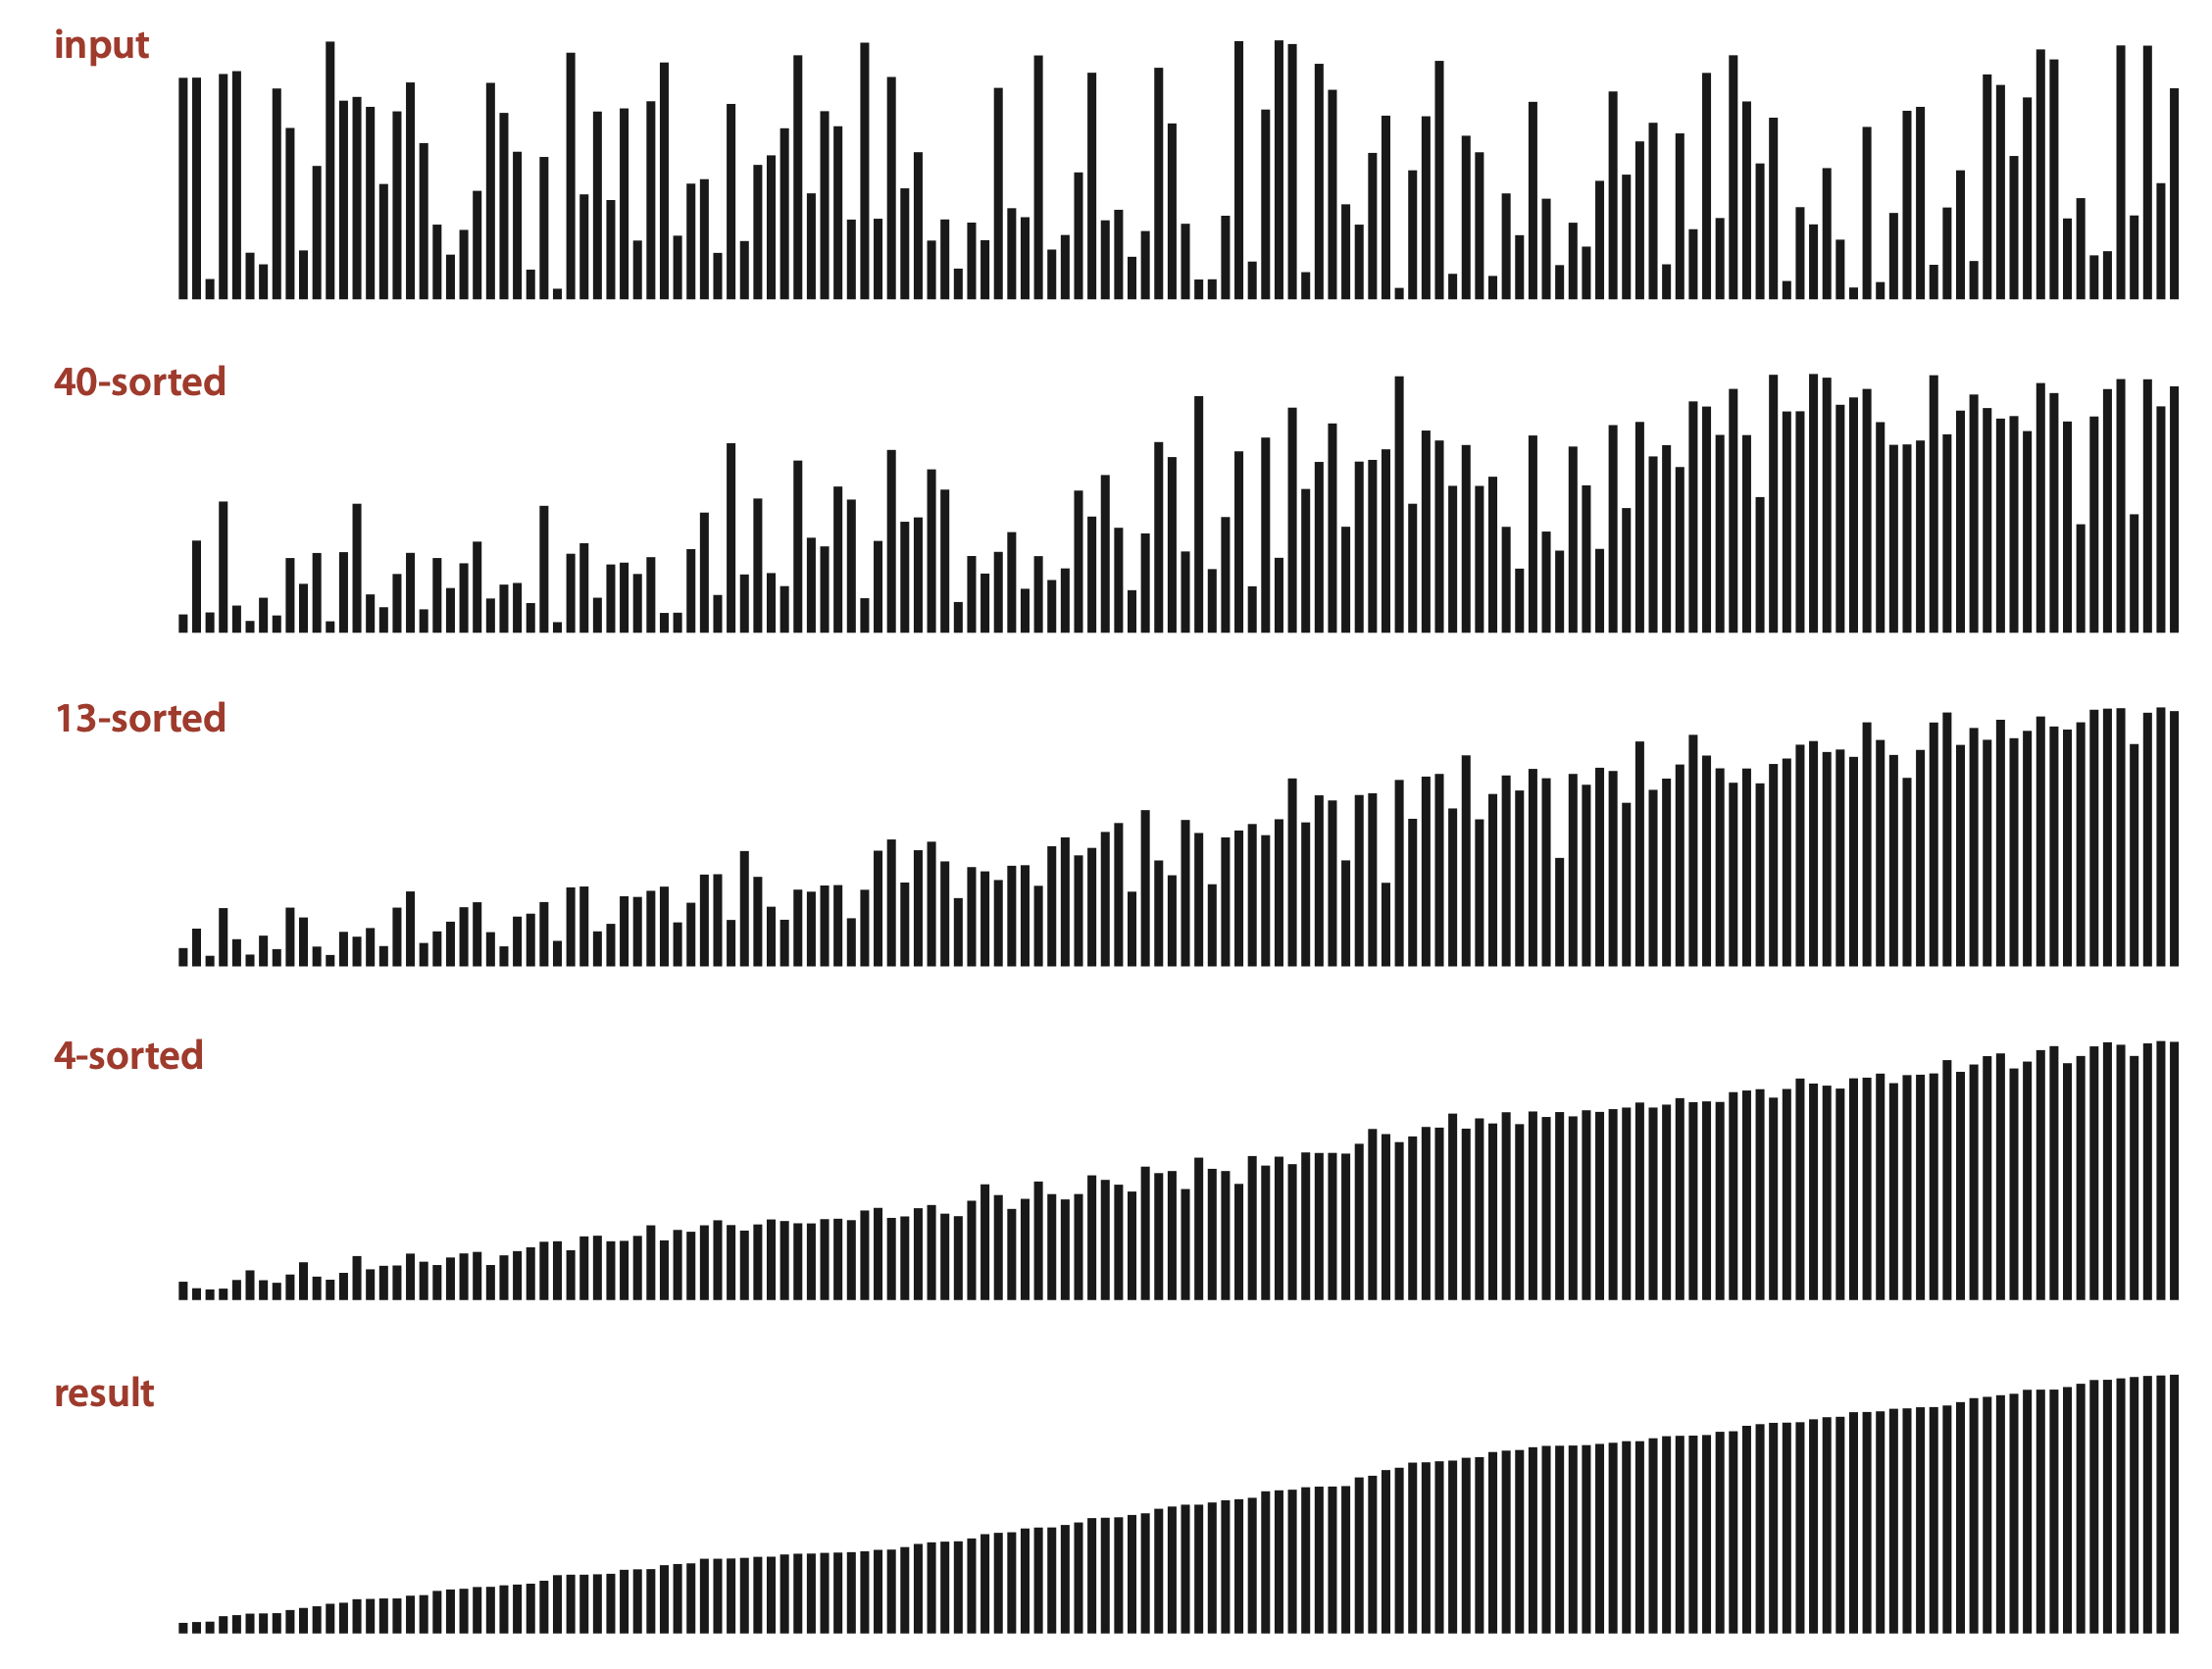
\includegraphics[width=10.5cm]{src/shellTrace.png}
    \caption{希尔排序轨迹图}
\end{figure}

\subsubsection{性能}
\begin{itemize}
    \item 希尔排序的时间复杂度与选定的 $\text{gap}$ 序列有关,最佳的 $\text{gap}$ 序列在学术界仍是开放问题。
    \item 本题选用的 $\text{gap} = 3 \times \text{gap} + 1$ 序列有 $O(n^{\frac{6}{5}})$ 的估计时间复杂度。
    \item 数据比较次数和移动次数与输入序列中个排序元素的初始排列有关。
    \item 希尔排序是不稳定的。
\end{itemize}

\section{快速排序}

\subsubsection{描述}
快速排序的核心思想是:让元素在切分中产生有序性。{\kaishu 切分}操作的意思是选定一个值作为 {\kaishu 枢纽(pivot)},将比枢纽小的元素%
放在枢纽左边,比枢纽大的元素放在枢纽右边,当切分到只有一个元素的时候,序列就是良序的。

\newpage

\begin{figure}[H]
    \centering
    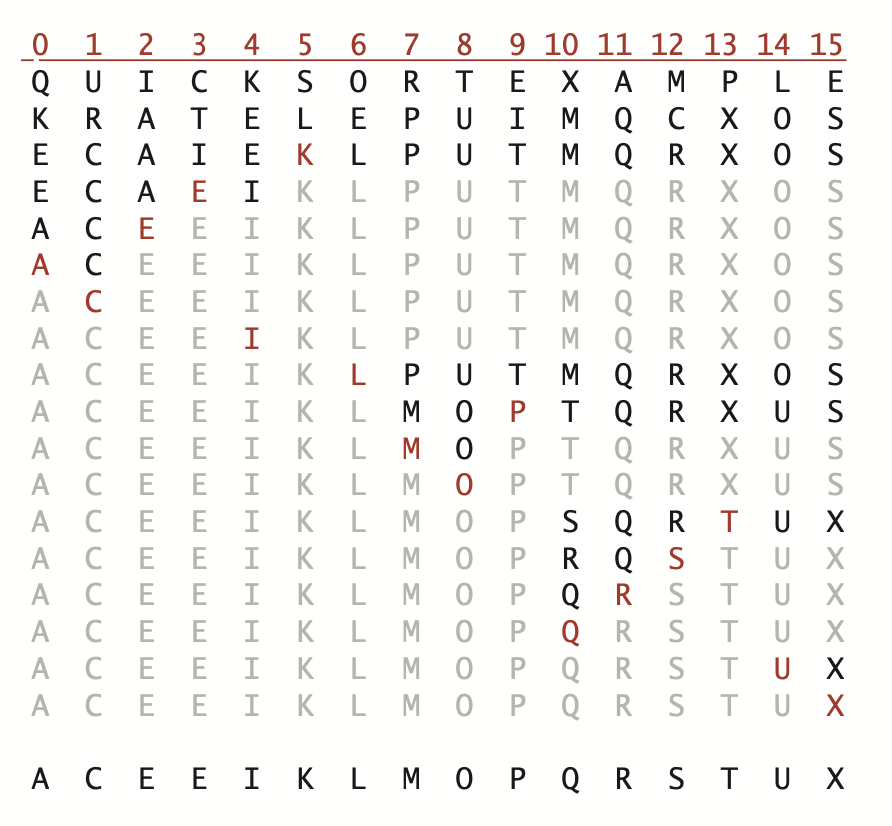
\includegraphics[width=10.5cm]{src/quick.png}
    \caption{快速排序示意图}
\end{figure}

\subsubsection{性能}
\begin{itemize}
    \item 堆排序的平均时间复杂度为$O(n\log_2{n})$ 。
    \item 数组有序或倒序的情况是最差情况,此时快速排序退化成 $O(n^2)$ 的算法,解决这个问题可以用不同策略选择枢纽,比如首尾中三个位置取中间数。
    \item 数据比较次数和移动次数与输入序列中个排序元素的初始排列有关。
    \item 快速序是不稳定的。
\end{itemize}

\section{堆排序}

\subsubsection{描述}
堆排序的步骤是:首先对根据初始数组建立最大堆,从下向上逐步调整为堆,此时第一个元素是序列中最大的。将第一个元素与序列尾部元素交换,%
序列尾部元素位置确定,再将第 $1$ 个到第 $n-1$ 个元素的子序列调整为堆(只需要一次下沉)、重复取出堆顶元素与子序列尾部交换,直至只剩一个%
元素剩余在头部,数组有序。

\newpage

\begin{figure}[H]
    \centering
    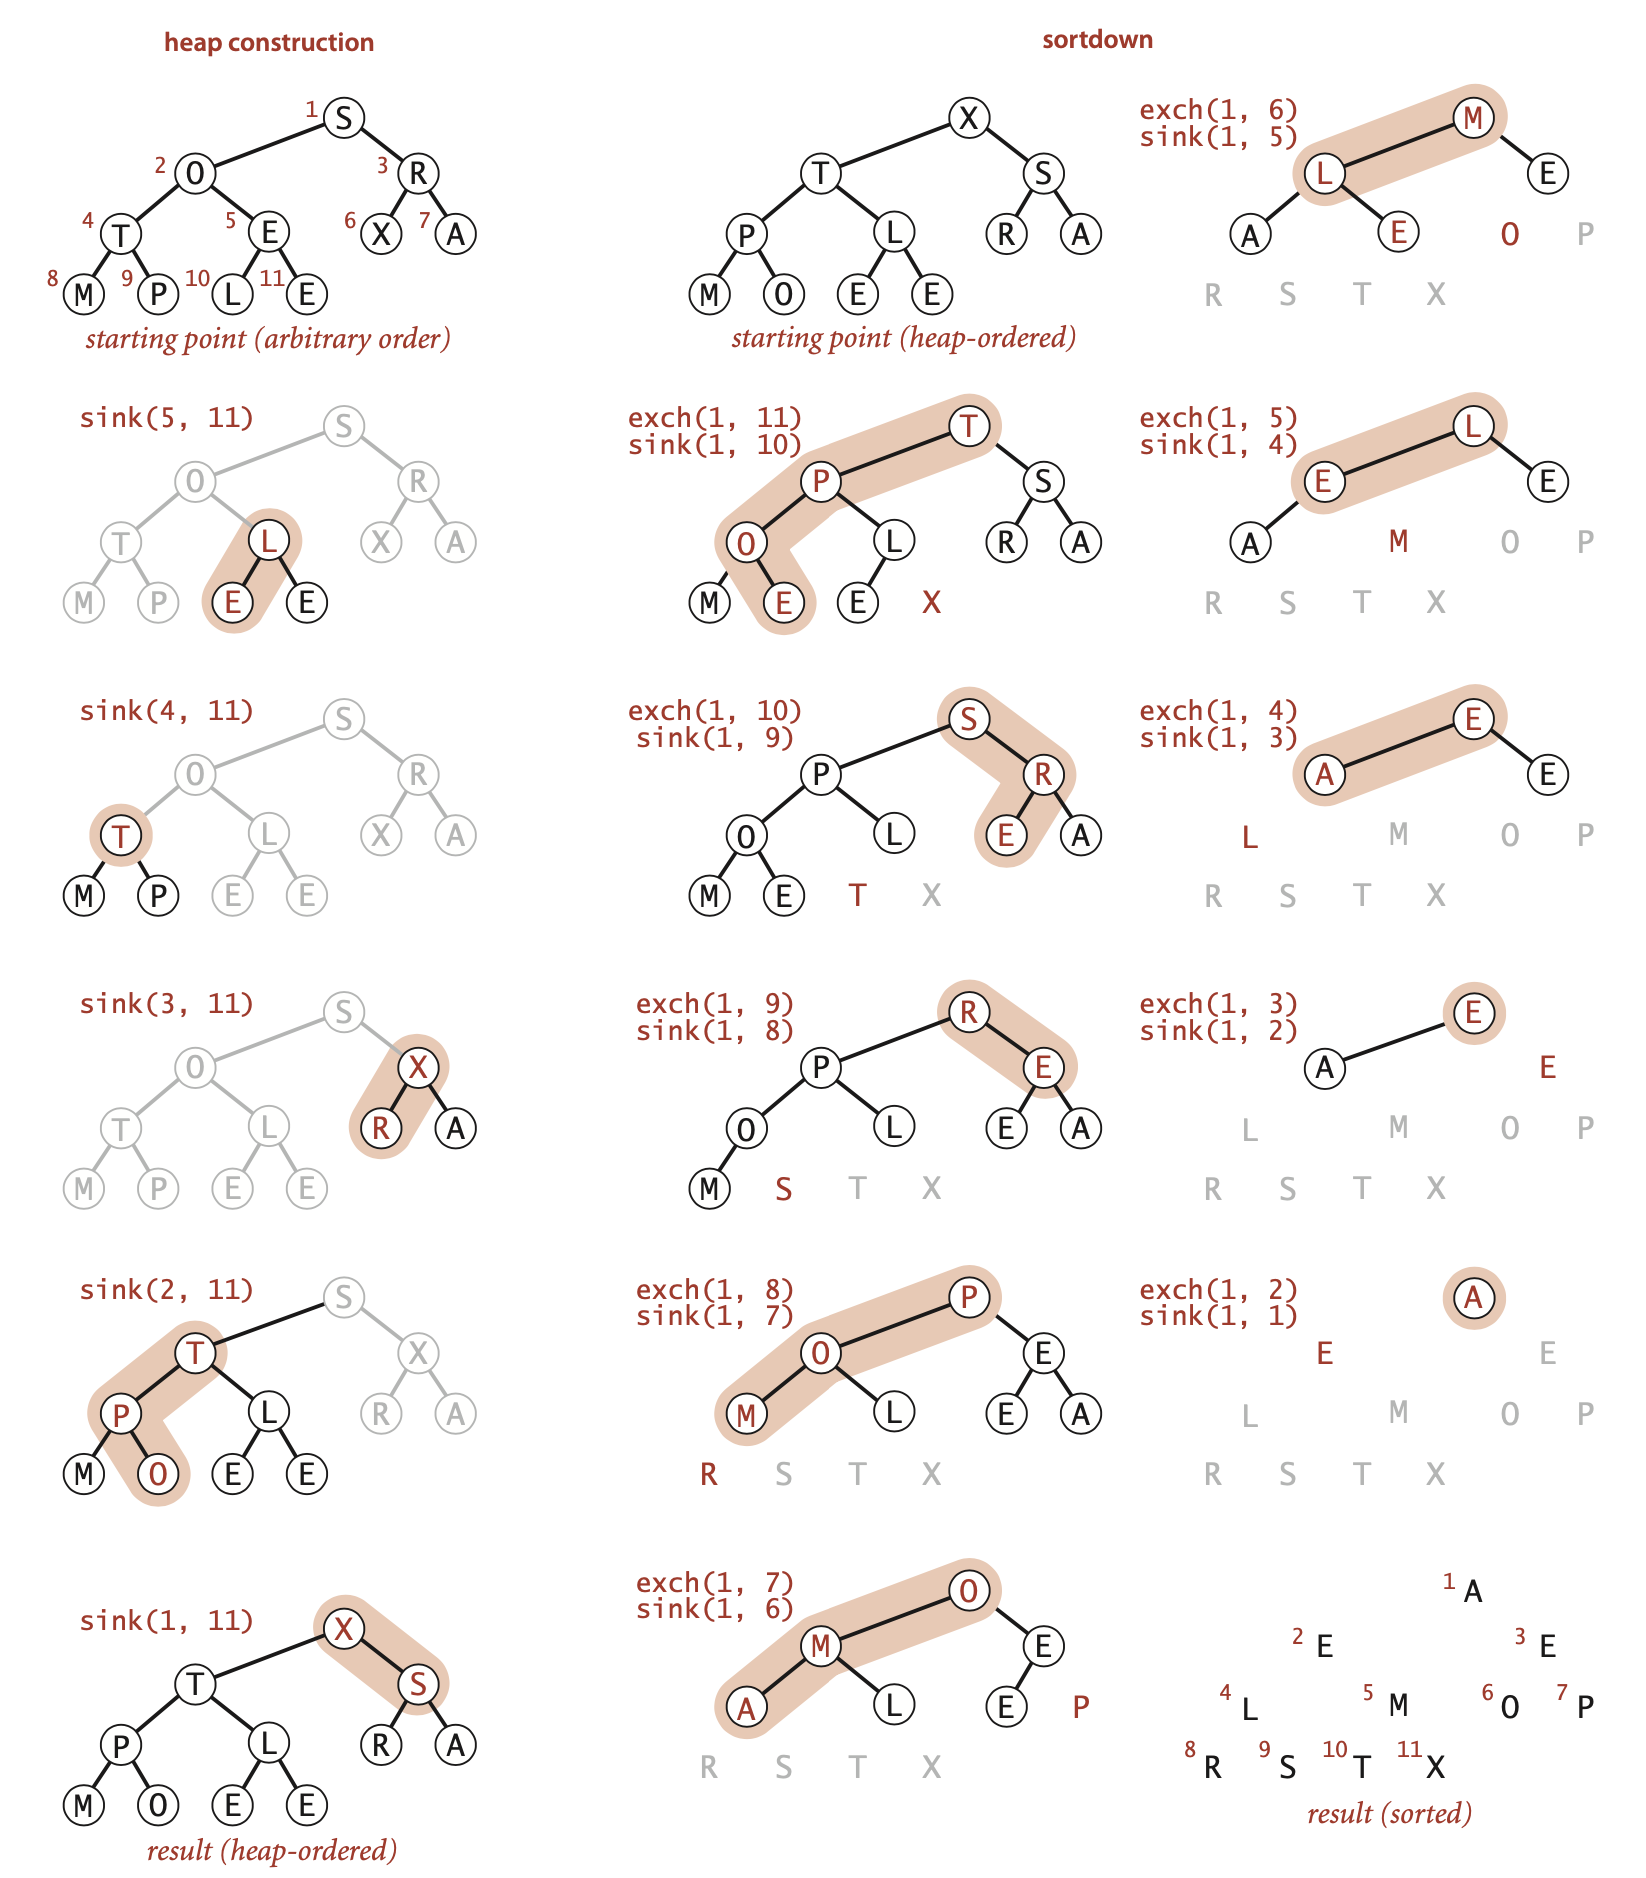
\includegraphics[width=14.5cm]{src/heap.png}
    \caption{堆排序示意图}
\end{figure}

\subsubsection{性能}
\begin{itemize}
    \item 堆排序的时间复杂度为$O(n\log_2{n})$ 。
    \item 数据比较次数和移动次数与输入序列中个排序元素的初始排列有关。
    \item 堆排序是不稳定的。
\end{itemize}


\section{归并排序}

\subsubsection{描述}
归并排序是一个将数组二分之后合并的排序,有两种方式:自底向上的和自顶向下的。

由于自底向上的实现方式不需要递归,这里介绍项目使用的自底向上的归并排序:开始时每个元素各自成一组,然后两两一组合并,%
小的元素先置入新数组,之后每次扩大分组的元素个数为两倍,每次取出要合并的两个数组头元素中小的那个置入新数组,直到分组的元素数量%
达到或大于数组长度。


\begin{figure}[H]
    \centering
    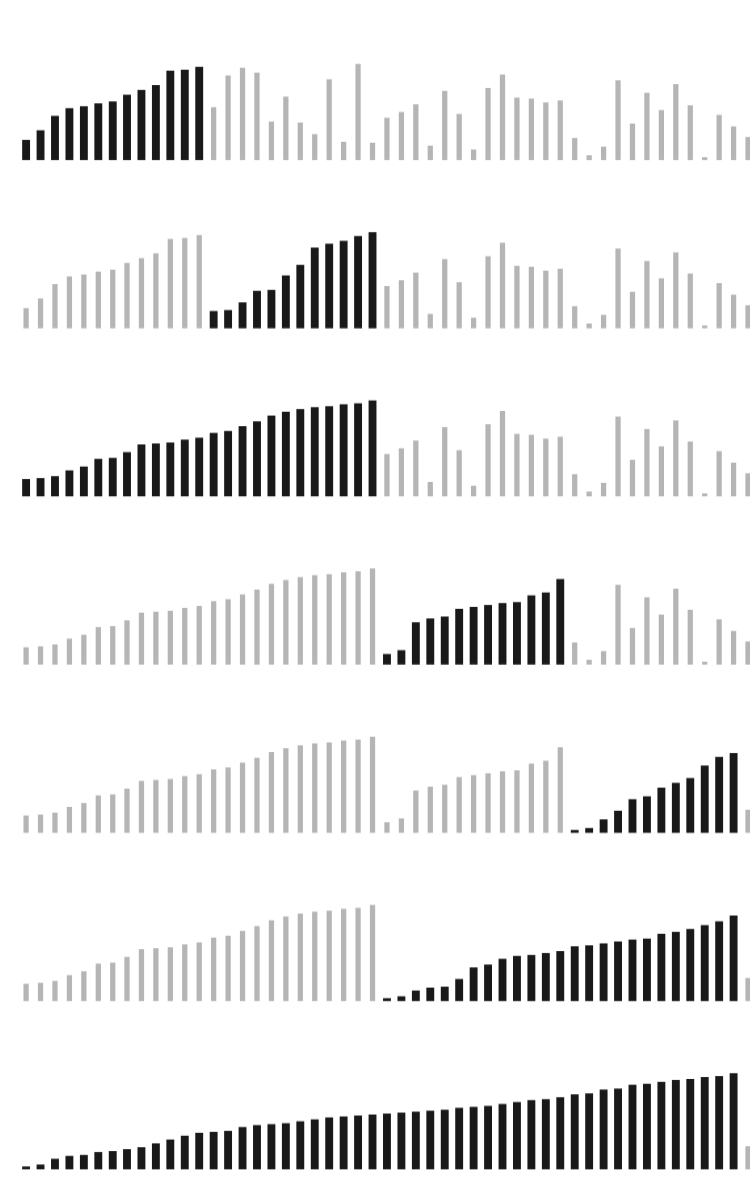
\includegraphics[width=12.5cm]{src/mergeTrace.png}
    \caption{归并排序轨迹图}
\end{figure}

\subsubsection{性能}
\begin{itemize}
    \item 堆排序的时间复杂度为$O(n\log_2{n})$ 。
    \item 数据比较次数和移动次数与输入序列中个排序元素的初始排列有关。
    \item 归并排序是稳定的。
\end{itemize}

\section{基数排序}

\subsubsection{描述}

选择一个数作为基数 $r$,从 $i = 0$ 开始,第i趟将待排数组里的每个数的i位数放%
到count[k]队列中(k 为 该数除 $r^{i-1}$ 之后对 $r$ 的余数),然后再从这两个%
队列中取出数据,重新放到原数组里,直到i大于待排数的最大位数 $\text{max}$。

\begin{figure}[H]
    \centering
    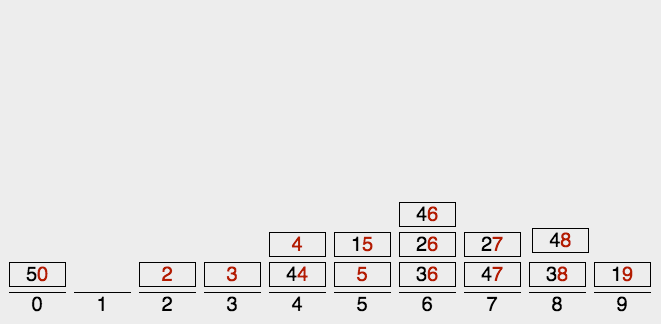
\includegraphics[width=12.5cm]{src/radix1.png}
    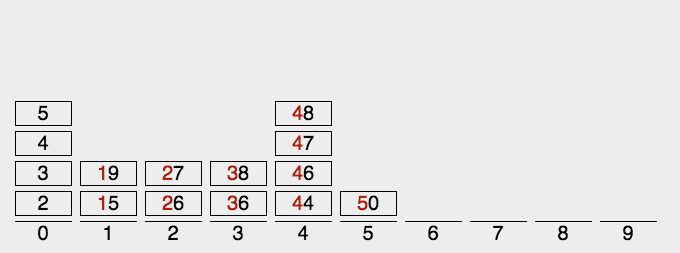
\includegraphics[width=12.5cm]{src/radix10.png}
    \caption{归并排序轨迹图}
\end{figure}

本题的基数排序是基于数组的,没有使用队列,每一次计数时都为本次处于 $nr$ 位置的元素留出空间,%
因此每次都要遍历两次序列。

\subsubsection{性能}
\begin{itemize}
    \item 基数排序的平均时间复杂度为 $O(n\log_r{\text{max}})$ 。
    \item 基数排序不是基于比较的排序,故其比较次数始终为0。移动次数与输入序列中个排序元素的初始排列无关,与序列中的最大值有关。  
    \item 基数排序是稳定的。
\end{itemize}

